 \begin{center}
 \textbf{
 %\dots
\og 
\og Ils sont justes passés de l’autre côté\fg{}
 \fg{}
 %\dots
 }
 \end{center}

Lorsqu’un être que nous aimons, qui nous est très proche, est emporté par la mort, nous disons que nous l’avons \og perdu \fg. Et nous avons l’impression désespérante que cette perte est définitive, que la mort est vraiment une fin. Nous disons alors volontiers que nous avons \og fait une perte irréparable \fg.

En effet, c’est toujours douloureux de perdre un être cher. Nul ne peut dire le contraire. Mais chrétiens ont imbus de la parole de Dieu, la foi chrétienne nous assure que les morts ressusciteront. Nous le disons même dans notre Credo :
\og Je crois\dots{} à la résurrection de la chair, à la vie éternelle \fg{}. Cette compréhension du Credo, doit nous aider à supporter l’épreuve présente.
Nous devons le croire, même si nous ne le voyons pas. Il nous faut donc nous laisser accabler par le souvenir de la fin douloureuse de celui que nous avons perdu. La foi doit nous aider à découvrir, sous ces apparences désolantes, la croissance invisible mais réelle d’un homme nouveau, qui se dégage peu à peu de cette épreuve pour acquérir son visage de beauté et d’éternité. C’est un peu la fleur qui, alors qu’elle se dessèche et flétrit, prépare le fruit brillant et savoureux qui se noue à partir d’elle. Ainsi la mort n’est pas seulement ce qu’elle parait :
diminution et destruction. Elle est en réalité transfiguration. Et c’est bien ce que nous reprenons dans la première préface des défunts où nous disons :
\og Pour tous ceux qui croient en toi, Seigneur, la vie n’est détruite, elle est transformée ; et lorsque prend fin leur séjour sur la terre, ils ont déjà une demeure éternelle dans les cieux. \fg{}

Dans l’espérance de la mort de ceux qui nous ont devancé, si nous sommes attentifs, ne nous oblige-t-elle pas en effet à regarder les choses autrement. Ainsi pour le croyant, la vie n’est pas détruite. Elle est transformée. Notre séjour sur terre est terminé mais alors s’ouvrent pour nous les portes d’une nouvelle demeure où il n’y a plus ni larmes, ni maladie et ni souffrance ; mais la paix et la joie.

\begin{wrapfigure}{l}{1.7cm}
\vspace{-0.4cm}
	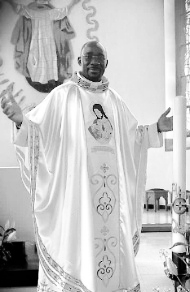
\includegraphics[scale=1.20]{../images/standing_daniel}
\end{wrapfigure}
Au cours ce mois de novembre que nous assemblées en soient déjà l’annonce et la préfiguration et que Dieu nous donne la joie de remarquer, autour de de nous, les petits signes qui montrent bien que notre prière est exaucée et que ce royaume arrive, qu’il est au milieu de nous et que bientôt nous aurons la claire vision de ce que nous espérons dans la foi.



\begin{flushright}
\textit{Père  Daniel  ETTÉ}
\end{flushright}

